%!TeX spellcheck = en-US, ru-RU
\documentclass[a4paper]{article}
\usepackage[warn]{mathtext}
\usepackage{amsmath}

\usepackage{cancel}
\usepackage[normalem]{ulem}

\usepackage[T2A]{fontenc}
\usepackage[utf8]{inputenc}
\usepackage[russian]{babel}

\usepackage[14pt]{extsizes}
\usepackage{graphicx}
\usepackage{wrapfig}
\usepackage{amssymb}
\usepackage{faktor}
\usepackage{multicol}
\RequirePackage{caption}

%\DeclarePairedDelimiter\floor{\lfloor}{\rfloor}

\DeclareCaptionLabelSeparator{defffis}{ : }
%\DeclareMathOperator{\tg}{tg}
%\DeclareMathOperator{\dif}{\mathbf{d}}
\captionsetup{justification=centering,labelsep=defffis}

% \usepackage[unicode, pdftex]{hyperref}
\usepackage{hyperref}
\hypersetup{
  colorlinks   = true, %Colours links instead of ugly boxes
  urlcolor     = blue, %Colour for external hyperlinks
  linkcolor    = blue, %Colour of internal links
  citecolor   = red %Colour of citations
}

\usepackage{setspace,amsmath}
\usepackage[left=20mm, top=15mm, right=15mm, bottom=15mm, nohead, footskip=10mm]{geometry} % настройки полей документа
\usepackage{graphicx}

\newcommand{\norm}[1]{\left\lVert#1\right\rVert}
\newcommand{\seg}[2]{\left[#1, \:#2\right]}
\renewcommand{\ch}[0]{\mathrm{ch}\,}
\renewcommand{\sh}[0]{\mathrm{sh}\,}
\newcommand{\dx}[0]{\,dx}
\newcommand{\ds}[0]{\,ds}
\renewcommand{\phi}{\varphi}
\renewcommand{\epsilon}{\varepsilon}
\renewcommand{\Re}[1]{\mathrm{Re}\left(#1\right)}
\renewcommand{\Im}[1]{\mathrm{Im}\left(#1\right)}

\newcommand{\task}[2]{A#1 $\Diamond$ #2}
\newcommand{\fact}[2]{\faktor{#1}{\left(#2\right)}}

\newcommand{\Deg}{^{\circ}}

\title{Листок №3}
\author{Кац Лев}

\setlength\parindent{0pt}

\begin{document}
  \maketitle

  \subsection*{\task{3}{1}}
  Пусть $g \in \mathbb{Q}\left[x\right]$.
  Тогда нам подходят:
  \begin{enumerate}
      \item $g \cdot (1 + x^2) + (1 + x)$
      \item $g \cdot (1 + x^4) + (1 + x^3)$
      \item $g \cdot (1 + x^8) + (1 + x^5)$
  \end{enumerate}

  \subsection*{\task{3}{3}}
  \subsubsection*{1.}
  Рассмотрим $\mathbb{F}^* = \mathbb{F} \setminus \{0\}$ -- мультипликативную подгруппу. Это конечная, а значит циклическая подгруппа ($\zeta$ -- порождающий).
  Построим функцию $\left[x=n\right]$ -- индикатор того, что $i = n$:
  $$\left[x=n\right] = 1 - (x - n)^{\mathrm{ord}\: \zeta},$$
  он равен $1$, если $x - n$ и $0$ иначе. Тогда:
  $$f(x) = \sum_{q \in \mathbb{F}} f(q)\left[x=q\right],$$
  это многочлен.
  \subsubsection*{2.}
  Пусть $f,\:g \in \mathbb{F}$ такие, что $\forall x \in \mathbb{F}\:f(x)=g(x)$. Рассмотрим многочлен $f - g$. Он равен нулю в каждой точке, то есть у него $|\mathbb{F}|$ корней. У нас степень многочленов (в 1) не превосходит $\mathrm{ord}\: \zeta = |\mathbb{F}| - 1$, а тогда $f - g = 0$.

  \subsection*{\task{3}{4}}
  От противного: пусть их конечный набор $f_1, ..., f_n$. Рассмотрим многочлен $g \equiv \prod_{k=1}^n f_k + 1$. Он дает остаток $1$ при делении на $f_k$ -- любой неприводимый многочлен. Однако $g$ можно разложить в произведение неприводимых многочленов, противоречие.

  \subsection*{\task{3}{5}}
  Перечислим их (для $2 \le \mathrm{deg}\: f \le 3$ достаточно подбирать те, у которых просто нет корней. Иначе нужно проверять делимость на неприводимые меньшей степени).
  \subsubsection*{а)}
  Понятно, что свободный коэффициент при степени больше $1$ будет равен $1$, а количество членов нечетным.
  \begin{itemize}
     \item $x$, $x + 1$;
     \item $x^2 + x + 1$;
     \item $x^3 + x^2 + 1$, $x^3 + x + 1$;
     \item $x^4 + x^3 + 1$, \sout{$x^4 + x^2 + 1 = (x^2 + x + 1)^2$}, $x^2 + x + 1$, $x^4 + x^3 + x^2 + x + 1$;
     \item \sout{$x^5 + x^4 + 1 = (x^2 + x + 1)(x^3 + x+ 1)$}, $x^5 + x^3 + 1$, $x^5 + x^2 + 1$,\\ \sout{$x^5 + x + 1 = (x^2 + x + 1)(x^3 + x^2 + 1)$},
     $x^5 + x^4 + x^3 + x^2 + 1$, $x^5 + x^4 + x^3 + x + 1$, $x^5 + x^4 + x^2 + x + 1$, $x^5 + x^3 + x^2 + x + 1$.
  \end{itemize}
  \subsubsection*{б)}
  \begin{itemize}
      \item $x^2 + 1$, $2x^2 + 2$
      \item $x^2 + x + 2$, $2x^2 + 2x + 1$
      \item $x^2 + 2x + 2$, $2x^2 + x + 1$
  \end{itemize}
  \subsection*{г)}
  Можем просто возвести элементы в квадрат:
  \begin{itemize}
      \item $\{0, 1\}$
      \item $\{0, 1, 4\}$
      \item $\{0, 1, 4, 7\}$
      \item $\{0, 1, 4, 9\}$
  \end{itemize}

  \subsection*{Лемма (я буду ее использовать в задачах):}
  $f \in \mathbb{Z}\left[x\right]$ имеет корень $p/q:\ \mathrm{gcd}(p, q) = 1 \Longleftrightarrow$ старший коэффициент делится на $q$, свободный -- на $p$
  \subsubsection*{Доказательство}
  \begin{eqnarray*}
    0 &=& a_0 \left(\frac{p}{q}\right)^n + ...+ a_{n - 1} \left(\frac{p}{q}\right)^1 + a_n \bigg{/} \cdot q^n \\
    -a_0 &=& q \left(a_1 p^n + ... + a_n q^{n - 1}\right) \\
    -a_n q^n &=& p \left(a_0 p^{n - 1} + ... + a_{n - 1} q^{n - 1}\right)
  \end{eqnarray*}

  \subsection*{\task{3}{6}}
  Будем использовать теорему о том, что для произвольного поля $\mathbb{K}$ $\mathbb{K} \left[x\right] / (f)$ -- поле $\Longleftrightarrow$ $f$ -- неприводим в $\mathbb{K}$.

  \subsubsection*{a)}
  $$x^4 + 1 = (x^2 - \sqrt{2}x + 1)(x^2 + \sqrt{2}x + 1)$$
  \subsubsection*{б)}
  $f$ является неприводимым. Иначе разложение выше на неприводимые было бы не единственным в $\mathbb{R}\left[x\right]$.

  Найдем обратный. Заметим, что $x^4 + 1 = (x + 1)(x^3 - x^2 + x - 1) + 2$, то есть $\left[0\right]_f = \left[x + 1\right]_f \cdot \left[x^3 - x^2 + x - 1\right]_f + \left[2\right]_f$. А тогда:
  $$\left[1\right]_f = \left[x + 1\right]_f \cdot \left(\left[x^3 - x^2 + x - 1\right]_f \cdot \left[0.5\right]_f\right) $$
  \subsubsection*{в)}
  $f$ является неприводимым, поскольку у него нет рациональных корней. Заметим, что $x^3+x+1=(x+1)(x^2-x+2)-1$ -- ура, сразу нашли обратный.

  \subsection*{\task{3}{7}}
  \subsubsection*{а)}
  Наш многочлен может быть представлен в виде произведения многочленов со степенями $2$ и $2$, либо $3$ и $1$ (невозможно, так как нет рациональных корней). Попробуем первый случай.
  \begin{eqnarray*}
    (a_0 x^2 + a_1 x + a_2) (x^2 + b_1 x + b_2) = a_0 x^4 + (a_0 b_1 + a_1)x^3 + (a_0 + 1 + a_1 b_1)x^2 +\\
    + (b_1 a_2 + a_1 b_2)x + a_2 b_2 = \\ = x^4 - 8 x^3 + 12 x^2 - 6 x + 2,
  \end{eqnarray*}
  получаем 5 уравнений, у которых нет рациональных решений, потому неприводим.
  \subsubsection*{б)}

  \subsection*{\task{3}{9}}
  \subsubsection*{а)}
  Пусть $b$ обратим:
  $$\nu(a) \le \nu(ab) \le \nu(abb^{-1}) = \nu(a) \Longrightarrow \nu(a) = \nu(ab)$$
  Пусть $b$ не обратим. Тогда $\exists\; p, r \in A: a = p(ab) + r,\:\nu(r) < \nu(ab)$. Тогда $a(1 - pb) = r$, тогда $\nu(a) \le \nu(a(1 - pb)) = \nu(r) < \nu(ab)= \nu(a)$, противоречие.
  \subsubsection*{б)}
  Рассмотрим $\{ax + by:\:x,y \in A\}$. В нем есть элемент $M \ne 0$ с наименьшей нормой (потому что это целые числа). Очевидно, он делится на любой общий делитель, при этом $\exists\; p, r \in A: a = pM + r,\: \nu(r) < M$. Если $r \ne 0$, то он будет одновременно лежать в множестве и противоречить выбору $M$, поэтому он $0$. Аналогично $M$ делится на $b$. Почему наибольшая норма? Пусть есть общий делитель с большей нормой. Тогда $M$ делится на него и значит имеет норму не меньше, противоречие.
  \subsubsection*{в)}
  Очевидно, на каждом шаге норма уменьшается, а потому шагов может быть только конечное число. Также из второго свойства понятно, почему в конце $r_{n + 1} = 0$ (в противном случае можно будет построить следующий элемент с меньшей нормой). Почему $r_n$ -- наибольший общий делитель? Заметим, что $\mathrm{gcd}(r_k, r_{k + 1}) = \mathrm{gcd}(r_{k+1}, r_{k + 2})$, поскольку обе пары имеют одинаковый набор общих делителей (по построению). Также заметим, что $\mathrm{gcd}(r_n, 0) = r_n = \mathrm{gcd}(a, b)$.

  \subsection*{\task{3}{10}}
  В качестве нормы возьмем целую часть от квадрата модуля комплексного числа, т.е
  $\nu(a) = \lfloor x\overline{x} \rfloor$. Для такой нормы очевидно выполнено первое свойство (в обоих пунктах):
  $$\nu(ab) \ge \lfloor a\overline{a} \rfloor \cdot \lfloor b\overline{b} \rfloor \ge \lfloor a\overline{a} \rfloor = \nu(a)$$
  Докажем второе свойство методом относительно долгого вглядывания в Рис 1. Конечно же, конкретные числа там подписаны только для наглядности, а важно там то, что $a$ оказывается в одном из квадратов или треугольников (или на стороне, что неважно).

  \begin{figure}[h]
  %\vspace{-5ex}
  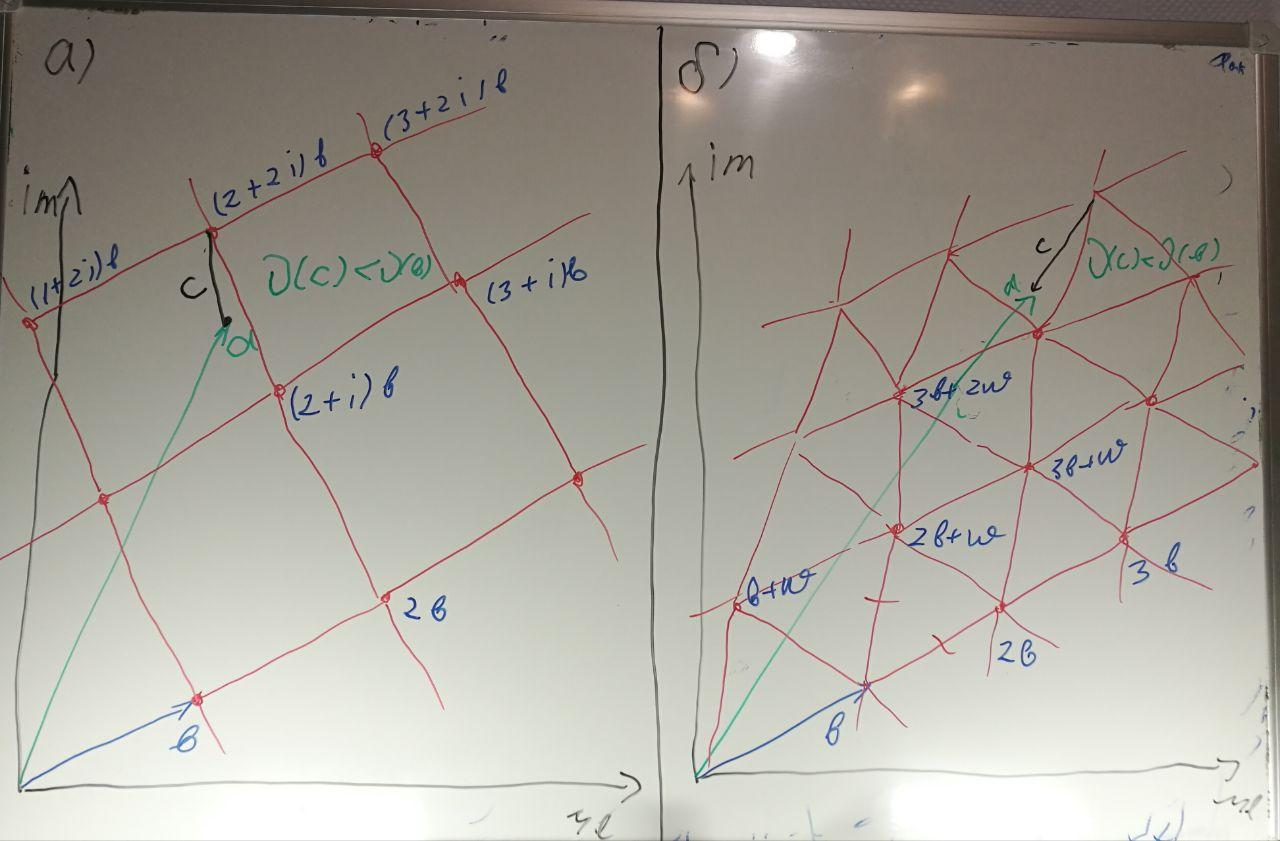
\includegraphics[width=\linewidth]{images/1.jpg}
  \caption{\task{3}{10}, доказательство свойства 2}
  \label{fig:somelabel}
  \end{figure}

  \subsection*{\task{3}{11}}
  Возьмем элемент $M \in I \setminus \{0\}$ с наименьшей нормой. Заметим, что $\forall \:b \in I\setminus\{0\} \: b = qM + r$, где $r = 0$, так как иначе в $I$ будет элемент с нормой $\nu(M)$. Заметим также, что кратные $M$ элементы содержатся в $I$, а тогда идеал главный.

  \subsection*{\task{3}{12}}
  $x,y \in \mathbb{Q}\left[x,y\right]$. Идеал, порожденный ими не может быть порожден одним элементом, тогда не является кольцом главных идеалов.

  Аналогично $x, 3 \in \mathbb{Z}\left[x\right]$.

  \subsection*{\task{3}{14}}
  \subsubsection*{а)}
  \begin{eqnarray*}
        z &=& (1 + i)^5/(1 - i)^3,\\
        |z|&=&\sqrt{2}^5 / \sqrt{2}^3 = 2,\\
        \mathrm{Arg}\:z &=& \frac{5\pi}{4} - \frac{3\pi}{4} + 2 \pi k = \frac{\pi}{2} + 2 \pi k,\\
        \Im{z} &=& 2,\\
        \Re{z} &=& 0.
  \end{eqnarray*}

  \subsubsection*{б)}
  \begin{eqnarray*}
        z &=& \left((\sqrt{3} + i)/(1 - i)\right)^{30},\\
        |z|&=& (2/\sqrt{2})^{30} = 2^{15},\\
        \mathrm{Arg}\:z &=& \frac{\pi}{6}\cdot 30 + 2\pi k = \pi + 2\pi k\\
        \Im{z} &=& 0,\\
        \Re{z} &=& -2^{15}.
  \end{eqnarray*}

  \subsubsection*{в)}
  \begin{eqnarray*}
        z &=& a + ib,\\
        |z|&=&\sqrt{a^2 + b^2},\\
        \mathrm{Arg}\:z &=& \arcsin\left(b/\sqrt{a^2 + b^2}\right), a\ge0\:\mathrm{else}\: \pi - \arcsin \left(b/\sqrt{a^2 + b^2}\right),\\
        \Im{z} &=& b,\\
        \Re{z} &=& a.
  \end{eqnarray*}

  \subsection*{\task{3}{15}}

  \begin{eqnarray*}
      \sin5\phi = \Im{(\cos\phi + i\sin\phi)^5} = \mathrm{Im}\left(\cos^5\phi + i\sin^5\phi + 5i\cos^4\phi\sin\phi + \right.\\
      \left.+ 5\sin^4\phi\cos\phi - 10\sin^2\phi\cos^3\phi - 10i\sin^3\phi\cos^2\phi\right) = \\
      = \sin^5\phi + 5 \cos^4\phi\sin\phi - 10\sin^3\phi\cos^2\phi =\\
      = 16\sin^5\phi - 20\sin^3\phi + 5\sin\phi
  \end{eqnarray*}
  Подставим $\phi = \frac{4\pi}{5}$ и обозначая за $x$:

  $$0 = x(16x^4 - 20x^2 + 5)$$

  Сделав замену $y = (4x^2 - 2.5)^2$ находим решение:

  $$x = 0,\: x = \pm\frac{1}{2}\sqrt{\frac{5}{2}\pm\frac{\sqrt{5}}{2}}$$

  В нашем случае $1 > \sin \phi > 0$, потому:

  $$\sin\frac{4\pi}{5} = \frac{1}{2}\sqrt{\frac{5}{2} - \frac{\sqrt{5}}{2}}$$

  Заметим, что $\cos\frac{2\pi}{5} = \sin\frac{\pi}{10}$. Просто в лоб подставить кажется сложным, поэтому попробуем выразить из $\sin\frac{\pi}{5}$, используя соотношение для косинуса двойного угла и тот факт, что $\sin\frac{\pi}{5} =  \sin\frac{4\pi}{5}$:

  $$\cos\frac{2\pi}{5} = 1 - 2\sin^2\frac{\pi}{5} = 1 - \left(\frac{5}{2} - \frac{\sqrt{5}}{2}\right) = \frac{\sqrt{5} - 1}{2}$$ 


  \subsection*{\task{3}{16}}
  Это циклическая группа, порожденная $\zeta$.

  \begin{eqnarray*}
      \sum_{i=0}^{n - 1} (\zeta^i)^s = \frac{\zeta^{ns} - 1}{\zeta - 1} = 0\\
      \prod_{i=0}^{n - 1} (\zeta^i)^s = \zeta^{s\sum_{i = 1}^{n - 1}} = \zeta^{1/2 (n - 1) n s} = 1
  \end{eqnarray*}
  \subsection*{\task{3}{17}}
  Заметим, что:
  $$(1 + i)^n = \sqrt{2}^n\left(\cos\left(\frac{\pi n}{4}\right) + i\sin\left(\frac{\pi n}{4}\right)\right) = \sum_{k=0}^n \binom{n}{k} i^k$$
  Также заметим свойство биномиальных коэффициентов:
  $$\binom{n}{0} + \binom{n}{2} + \binom{n}{4} + ... = \binom{n}{1} + \binom{n}{3} + ... = 2^{n - 1}$$
  Тогда:
  \begin{eqnarray*}
       \frac{\Re{(1 + i)^n}+ 2^{n - 1}}{2} = \frac{\sqrt{2}^n\cos\left(\frac{\pi n}{4}\right) + 2^{n - 1}}{2} = \binom{n}{0} + \binom{n}{4} + \binom{n}{8} + ...\\
       \frac{\Im{(1 + i)^n}+ 2^{n - 1}}{2} = \frac{\sqrt{2}^n\sin\left(\frac{\pi n}{4}\right) + 2^{n - 1}}{2} = \binom{n}{1} + \binom{n}{5} + \binom{n}{9} + ...
  \end{eqnarray*}
  Это немного контринтуитивно для меня, но как и ожидалось, числа получаются целыми положительными для любых $n$.


\end{document}
